\chapter{Introduction}
\label{chapterlabel1}
\section{Charge Transport Regimes in Organic Semiconductors}
\subsection{Organic Semiconductors}
Conductive polymers were first discovered in 1977 by Shirakawa et al  \cite{chiang_electrical_1977, Shirakawa1977Jan} for which they were awarded the Nobel prize in Chemistry. Recently these materials have become ubiquitous in many technologies, such as in organic solar cells\cite{Kippelen2009}, organic field-effect transistors (OFET) \cite{Malachowski2010Jun} and organic light-emitting diodes (OLED) \cite{ThejoKalyani2012Jun}. While the other two technologies lag behind their inorganic counterparts, uptake of OLED screens is becoming increasingly popular -especially in the smartphone and television market due to their flexibility, better colour reprsentation and lower energy consumption than standard backlit LCD displays. In fact IHS markit's OLED market tracker predicts OLED to be the dominant technology in smartphone screens by 2020 \cite{IHSMarkit}. OLEDs have also found uses in lighting with their efficiency rivalling that of fluorescent tubes \cite{Reineke2009May, OLED_lighting}. Although, industry has made large strides in fabricating and using these materials the exact nature of the charge transport is still poorly understood. Conventional hopping and band theories break down in the regime of partial delocalisation of the charge carriers and atomistic simulations are required for a realistic picture.
\\\\
Typically charge carrier mobilities in `good' organic semiconductors (OSCs) fall between 1-10 cm$^2$ V$^{-1}$s$^{-1}$ \cite{Brown2018Mar}. This is just beyond the range of hopping model validity ($\sim $ 1 cm$^2$ V$^{-1}$s$^{-1}$ ) and below that of band theory ($>$ 50 cm$^2$ V$^{-1}$s$^{-1}$ )
 \cite{yavuz_dichotomy_2017}. In this intermediate regime the charge carriers are typically not completely delocalised at the valence band edges (band regime) or localised to a single site/molecule (hopping regime) but delocalised over a few molecules. Without any analytic approaches currently being valid in this regime many computational approaches have been developed to investigate the underlying charge transport mechanisms \cite{oberhofer_charge_2017}.
%\subsection{Band-like Transport}
%For high mobility, inorganic, semi-conducting materials such as Silicon and Germanium some variation on band theory can be applied. As large numbers of atoms come together to form a crystal their atomic orbitals overlap \cite{AshcroftNeilW1976Ssp}. Due to the Pauli exclusion principle the energy level of the orbitals have to split to prevent any atoms having the same four quantum numbers. In a crystal with many atoms this splitting produces bands of energy separated by tiny values, effectively creating a continuum. In an inorganic semiconducting crystal the lattice sites (ions) are positively charged and create a periodic potential. Bloch's theorem can therefore be applied and the Schr\"odinger equation can be solved (with some approximations) to find the allowed energy bands. In general, these allowed bands form to produce a forbidden band in which there are no energy levels. This is called the band gap.
%\\\\
%The two important bands for charge transport in semiconductors are the conduction and valence bands. These are the 2 bands either side of the Fermi level -the energy level, at thermodynamic equilibrium, which has a 50\% chance of being populated. In order to conduct, a material must have empty states for electrons to move into. Those with no empty states are called insulators. In terms of band theory this means that the band-gap between the valence and conduction bands is very large; resulting in totally full states in the valence band and totally empty states in the conduction band \cite{KittelCharles1996Itss}. For a conductor the Fermi level is somewhere in the valence band making it partially full. This results in plenty of free states for the electrons to move into without having to cross a band gap. Semiconductors on the other hand do have a band gap but it is small enough to be overcome by thermal fluctuations. This puts conductivity in these materials somewhere between an insulator and conductor.
%\\\\
%Although successful in describing mobilities in inorganic semiconducting materials the assumptions of band theory make its use fairly limited in most inorganic crystals. The validity of band theory is linked to the delocalisation of charge carriers across the material \cite{oberhofer_charge_2017}. In many organic semiconductors the charge carrier is only partially delocalised. For Bloch's theorem to hold the crystal must be periodic and uniform throughout. However, many organic crystals show some disorder \cite{Habgood2011May, Vehoff2010Aug, Brown2018Mar}. Further the periodic potential felt by the electrons is assumed to be static and doesn't interact with phonons and other electrons etc... This requirement is often not fulfilled in organic semiconductors as the molecules comprising the crystal are often only held together with weak Van Der Waals forces and a fairly free to move around.
%\subsection{Hopping-like Transport}
%Hopping theories assume the charge carrier is localised on one site and can hop from site to site in a series of discrete hops \cite{oberhofer_charge_2017}. There are various underlying mechanisms for this. For example, the presence of the charge carrier at a site can alter the nuclear geometry. This distorted nuclear geometry can make it harder for the charge carrier to move onto the next site, creating a metastable state and trapping the charge carrier. The deformation in the nuclear geometry is called a small polaron.
%\\\\
%Polaronic hopping theories have been used to great success with rates provided by Marcus theories and their derivatives \cite{Gajdos2013Mar, Marcus1985Aug}. One of the key tools used in visualising this process (assuming harmonic response) are the Marcus Parabolas. These show how the free energy and reaction coordinates change after a charge transfer i.e. from initial to final diabatic states. The term `diabatic state' isn't well defined and can refer to different things in different formulations. In this work a diabatic state can be imagined as the charge carrier localised on a single molecule. This is discussed later in more detail in section \ref{chap:FOB}\\
%\\
%\begin{figure}[ht]
%  \includegraphics[width=\textwidth]{./img/diabatic_wells.png}
%  \caption{Marcus parabolas depicting the relationship between the free energy in the system and the reaction coordinate at 0 electronic coupling. This figure was taken from Oberhofer et al \cite{oberhofer_charge_2017}}
%  \label{fig:diab_wells}
%\end{figure}
%\\
%Figure \ref{fig:diab_wells} above defines various important quantities for calculating the mobility in materials displaying hopping-like transport. The initial parabola describes the change in free energy with respect to the reaction coordinate for the initial state, for example when the charge is located on site 1. The final parabola describes the change in free energy when the charge is located on site 2 e.g. when the charge has relocated to site 2. The transition state (TS) is a point where the energies of the initial and final states are the same. This degenerate point is the only point at which the charge can move from the initial to final state as other points would result in a non-zero jump in energy between the 2 parabolas. The diabatic activation energy $\Delta G^{\ddagger}$ defines the energy required to get to this transition state from the minima of the initial parabola. The driving force $\Delta G^{0}$ is the difference in minima of the 2 parabolas, the reorganisation energy $\lambda$ defines the energy required to change the reaction coordinate from the final state minima to the initial state minima without changing electronic state.
%\\\\
%Figure \ref{fig:diab_wells} can change when there is a non-zero electronic coupling ($H_{ab}$) between diabatic states. This parameter increases the chance of moving between the initial and final diabatic states by lowering the diabatic activation energy i.e. the energy required to transition from state 1 to 2. This is visualised in figure \ref{fig:adiab_wells}
%\begin{figure}[ht]
%  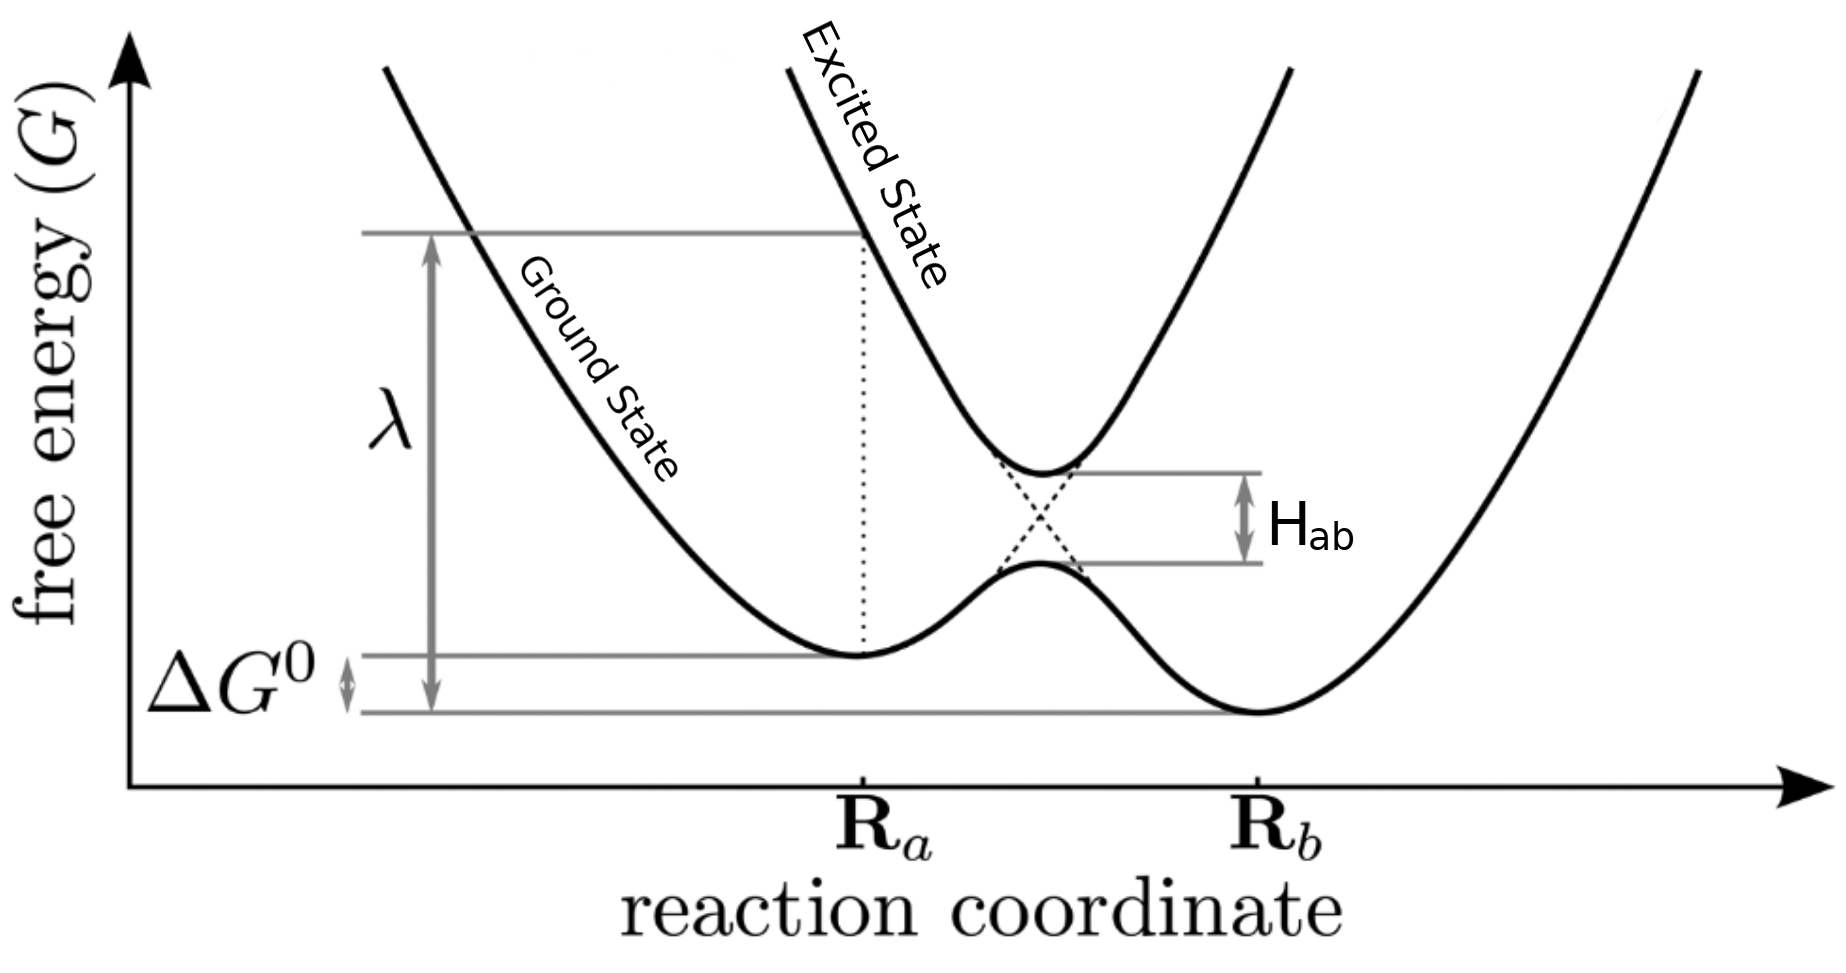
\includegraphics[width=\textwidth]{./img/adiabatic_wells.png}
%  \caption{Graph depicting the change in free energy for a change in reaction coordinate for non-zero electronic coupling. Adapted from \cite{oberhofer_charge_2017}}
%  \label{fig:adiab_wells}
%\end{figure}
%In figure \ref{fig:adiab_wells} above the diabatic activation energy has be lowered to $\Delta G^{\dagger} = \Delta G^{\ddagger} - H_{ab}$ making it easier for charge carriers to transition between diabatic states. In our formalism this means it is easier for charge carriers to move between sites i.e. delocalise. We see also that instead of being described totally by 2 parabolas there are 2 new adiabatic potential energy surfaces arising -the ground and excited state. The amount that these new potential energy surfaces diverge from the diabatic wells is dependent on an adiabaticity factor which is proportional to the ratio between the electronic coupling, $H_{ab}$, and the re-organisation energy, $\lambda$. This has been discussed in detail in multiple papers \cite{oberhofer_charge_2017, spencer_fob-sh:_2016, spencer_confronting_2016,   Gajdos2013Mar} .
%\\\\
%In fact for systems with couplings larger than $H_{ab} > \frac{3}{8} \lambda$ the diabatic activation energy vanishes completely \cite{Gajdos2013Mar}, meaning that there is no energy cost in transitioning between diabatic states. Beyond this regime hopping theories cannot be accurately applied. Unfortunately, at room temperatures thermal flucuations means the mean free path of the charge carriers is comparable to the intermolecular spacing. As such band theories too are inapplicable
%\cite{oberhofer_charge_2017, gajdos_ultrafast_2014, Gershenson2006Sep}. Much beyond this regime the energy cost to transition to higher adiabatic potential energy surfaces becomes prohibitively high and the system travels on a single state. In these situations the Born-Oppenhiemer approximation is valid. However, in this work I will be looking into the regime in between the band and hopping-like transport where we currently don't have  analytical theories to describe charge transport. For this I will be using non-adiabatic atomistic simulations, namely coupled-trajectory mixed quantum classical molecular dynamics (CTMQC).
%\newpage
\section{Atomisitc Simulations of Nonadiabatic Processes}
In simulating processes involving electronic transfers a key approximation used in conventional molecular dynamics (MD) breaks down. That is the Born-Oppenheimer or adiabatic approximation \cite{john_c._tully_nonadiabatic_nodate}. This approximation, relied upon for almost a century \cite{Pisana2007Feb}, hinges on the fact that nuclei are more massive than electrons and are approximately stationary with respect to electron movement \cite{Born1927Jan}. This results in nuclear evolution that is governed by a single, adiabatic, potential energy surface. However, in many interesting processes, such as electron transfer, non-radiative decay and photochemical processes, electronic transitions between adiabatic potential energy surfaces occur \cite{tully_nonadiabatic_1991}. Simulating these processes requires non-adiabatic molecular dynamics (NAMD) techniques to be developed, to correctly capture dynamical properties.
\\\\
There have been many techniques proposed for use in NAMD such as the quantum classical Louiville equation \cite{Kapral1999May}, multiple spawning \cite{Martnnez*2005Oct} or nonadiabatic Bohmian dynamics \cite{Albareda2014Aug}. However, two of the most popular are trajectory surface hopping \cite{Tully1990Jul} and mean-field approaches \cite{Whetten85}. This is probably due to their relative simplicity to implement, efficiency for large systems and proven efficacy in a wide variety of situations. In these approaches the general aim is to treat as much of the system as possible with (computionally cheaper) classical mechanics. While handling all necessary parts with quantum mechanics \cite{Coker1995Jan}. In Surface Hopping, Ehrenfest and CTMQC one treats the nuclear subsystem classically and the electronic one quantum mechanically. The nuclei are propagated using a velocity verlet algorithm according to Newton's laws. The electrons are propagated using a fourth order Runge Kutta algorithm according to the time-dependent Schr\"odinger equation. This is normally expanded as a linear combination of adiabatic or diabatic states. The nuclei and electrons can also interact. Taking account of this interaction is where these different atomistic simulation techniques differ. Both trajectory surface hopping (SH) and Ehrenfest have significant downsides that the new algorithm CTMQC aims at overcoming with minimal computational overheads. In this project I will be developing an efficient implementation of CTMQC within the CP2K code.
\newpage
\subsection{Surface Hopping and Ehrenfest Dynamics \label{sec:Ehren_SH}}
\begin{wrapfigure}{r}{0.45\textwidth}
  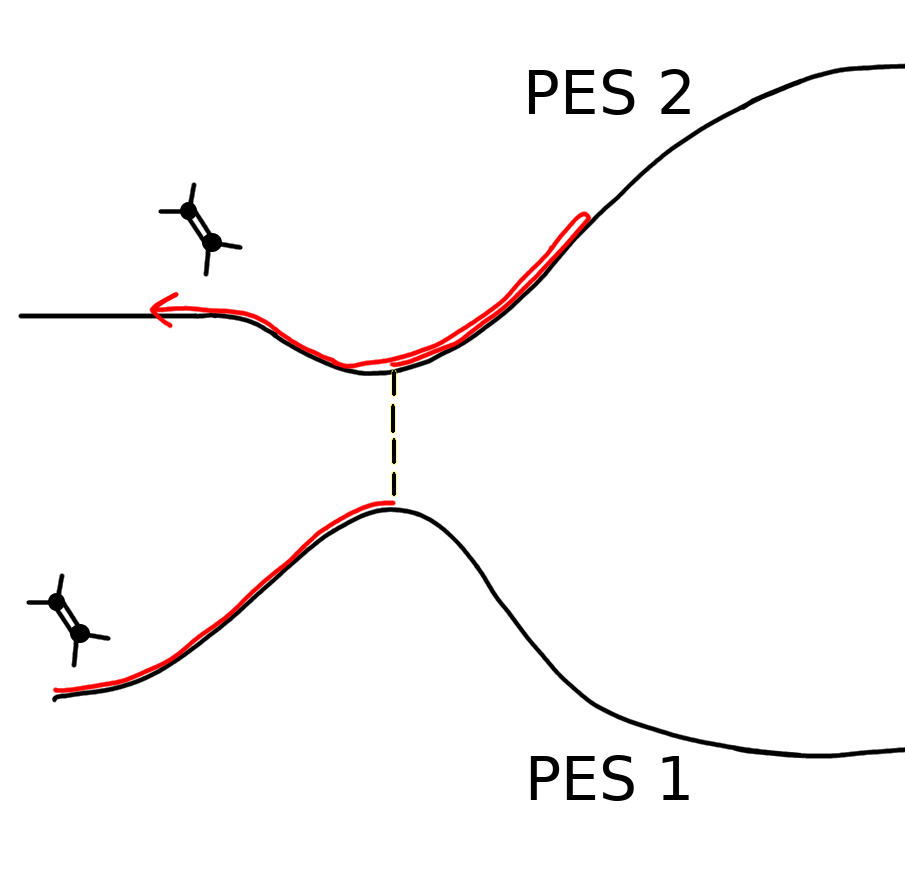
\includegraphics[width=0.45\textwidth]{./img/SH_hop.png}
  \caption{\label{fig:SH_diag}An example of a surface hopping simulation near an avoided crossing with a hop. The black lines represent the adiabatic potential energy surface due to the ground and first excited state. The red line represents the effective potential the ethylene molecule feels as it is propagated.}
\end{wrapfigure}
In surface hopping, Ehrenfest and CTMQC dynamics the effect of the electrons on the nuclei is felt through the potential energy surface. In short, the electronic populations control how the potential energy surface looks. This in turn controls the motion of the nuclei through $F = -\nabla E$. This method relies on a swarm of trajectories with slightly different initial conditions to sample configuration space. In this way branching of the nuclear wavepacket can be captured as different trajectories can travel on different potential energy surfaces.
\\\\
In surface hopping the shape of the potential energy surface is determined by a series of discrete stochastic hops between adiabatic potential energy surfaces \cite{tully_perspective:_2012}. See fig \ref{fig:SH_diag}.  The probability of these hops is determined by the non-adiabatic coupling between states. If this is high then a higher proportion of the total trajectories will hop if this is low then very few will. Although this method has been extremely successful, it has a few shortcomings. The original `fewest switches surface hopping' proposed by John Tully suffered from bad overcoherence of the nuclear and electronic subsystems. That is the electronic and nuclear motion was coupled long after the region of high non-adiabatic coupling (crossing region). The fact that the hops are instant leads to discontinuities and methods need to be implemented to fix these such as velocity re-scaling. Finally, perhaps the most important shortcoming is that this technique has not been derived from first principles and cannot be guaranteed to work generally. These problems have lead to a number of other techniques being developed.
\newpage
\begin{wrapfigure}{r}{0.45\textwidth}
  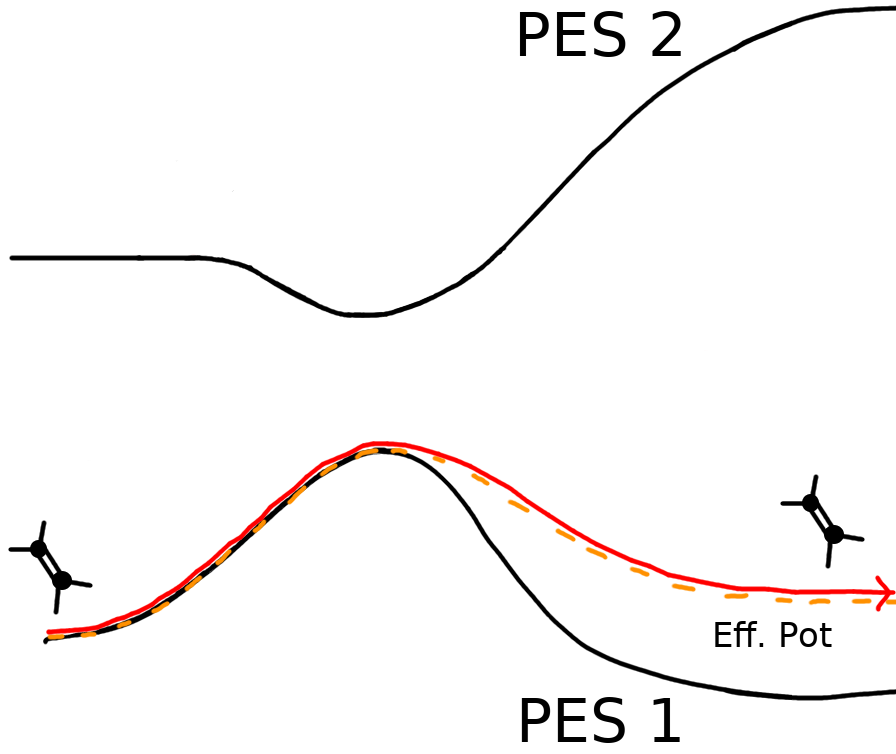
\includegraphics[width=0.45\textwidth]{./img/Eh_hop.png}
  \caption{\label{fig:Eh_diag}An example of a typical Ehrenfest simulation near an avoided crossing. The black lines represent the adiabatic potential energy surface due to the ground and first excited state. The red line represents the population weighted average potential the ethylene molecule feels as it is propagated.}
\end{wrapfigure}
\noindent Another popular technique in the field of non-adiabatic dynamics is Ehrenfest dynamics (see fig \ref{fig:Eh_diag}). In this the nuclei travel on a potential energy surface that is a electronic population weighted average of the adiabatic potential energy surfaces. The electronic propagation is the same as in surface hopping. This technique, although derived from first principles, has a number of shortcomings of its own. The splitting of the nuclear wavefunction at crossing regions cannot be captured in Ehrenfest, as each trajectory will be travelling on a slightly different average potential energy surface. Just as important is the fact that Ehrenfest violates detailed balance \cite{tully_perspective:_2012, john_c._tully_nonadiabatic_nodate}. In fact it has been shown that Ehrenfest will populate all adiabatic states
equally \cite{parandekar_detailed_2006}. This can lead to an infinite electronic temperature in the limit of infinite electronic states.

\subsection{Motivation for my Work}
To overcome some of the challenges of the traditional Ehrenfest and Surface Hopping simulation techniques I plan to implement the newly proposed CTMQC technique \cite{agostini_quantum-classical_2016}. This has been rigorously derived from the exact factorisation of the molecular wavefunction \cite{abedi_exact_2010} and has been shown to work for toy model systems and a single molecule of Oxirane \cite{abedi_dynamical_2013, agostini_quantum-classical_2016}. The equations appear to be the standard Ehrenfest equations with a correction provided by 2 new terms -the quantum momentum and a time-integrated adiabatic force. This correction allows a more theoretically rigorous handling of the decoherence and nuclear wavepacket splitting seen in nonadiabatic systems.
\\\\
This technique should not be much more expensive than either surface hopping or Ehrenfest and when paired with a FOB formalism (see section \ref{chap:FOB}) it should roughly scale as $\mathcal{O}(N_{mol}^3)$. Where $N_{mol}$ is the number of molecules in the system. 
